\documentclass[12pt,a4paper]{article}
\usepackage{amsmath}
\usepackage{amsfonts}
\usepackage{amssymb}
\usepackage{graphicx}
\usepackage{secdot}
\usepackage{multirow}
\usepackage[left=2cm,right=2cm,top=2cm,bottom=2cm]{geometry}

\title{{Experiment - 8\\ \textbf{Drag estimation on symmetrical airfoil NACA0015 from wake profile measurent}}}
\author{Arka Pramanick, AE21B007\\ Department of Aerospace Engineering\\ IIT Madras\\[3ex] Instructor:\\ \large Professor Dr. R. Sriram}

\date{10 April, 2023}


\begin{document}
\maketitle

\hline

\section{Aim :}
\begin{itemize}
    \item To estimate Drag from wake velocity profile measurement.
    \item To observe variation of Coefficients of Drag with Angle of Attack on increasing velocity.
\end{itemize}


\section{Apparatus :}
Required apparatus for performing this experiment are:
\begin{itemize}
    \item Manometer
    \item C15-10 Armfield tunnel
    \item Pitot-static Probe
    \item Fan
    \item Symmetrical Airfoil model
\end{itemize}



\newpage
\section{Theory :}

\underline{\textbf{Drag}} : Drag is the force which opposes the motion of an object.
Drag is calculated by : \\
$$D = \int_{-\infty}^{\infty} \rho v (V_{\infty}-v)\,dy $$
\underline{\textbf{Coefficients of Drag }} :
Drag coefficients caused due to skin friction and Drag. Drag coefficients is calculated by :
$$ C_d = \frac{2D}{(\rho V_{\infty}^2 d)/2} $$ \\
\underline{\textbf{Stagnation and Static Pressure :}}
Stagnation pressure is the pressure at the stagnation points in the fluid flow.Static pressure is the actual thermodynamic pressure of a flow.
$$  P_{stag} = P_{\infty} + \frac{\rho v^2}{2} $$
\underline{\textbf{Reynolds Number :}}
The Reynolds number is the ratio of inertial forces to viscous forces within a fluid which is subjected to relative internal moment due to variation of velocities.
$$  R_e = \frac{\rho V_{\infty d}}{\mu} $$
\begin{figure}[!ht]
	\begin{center}
		\framebox{
			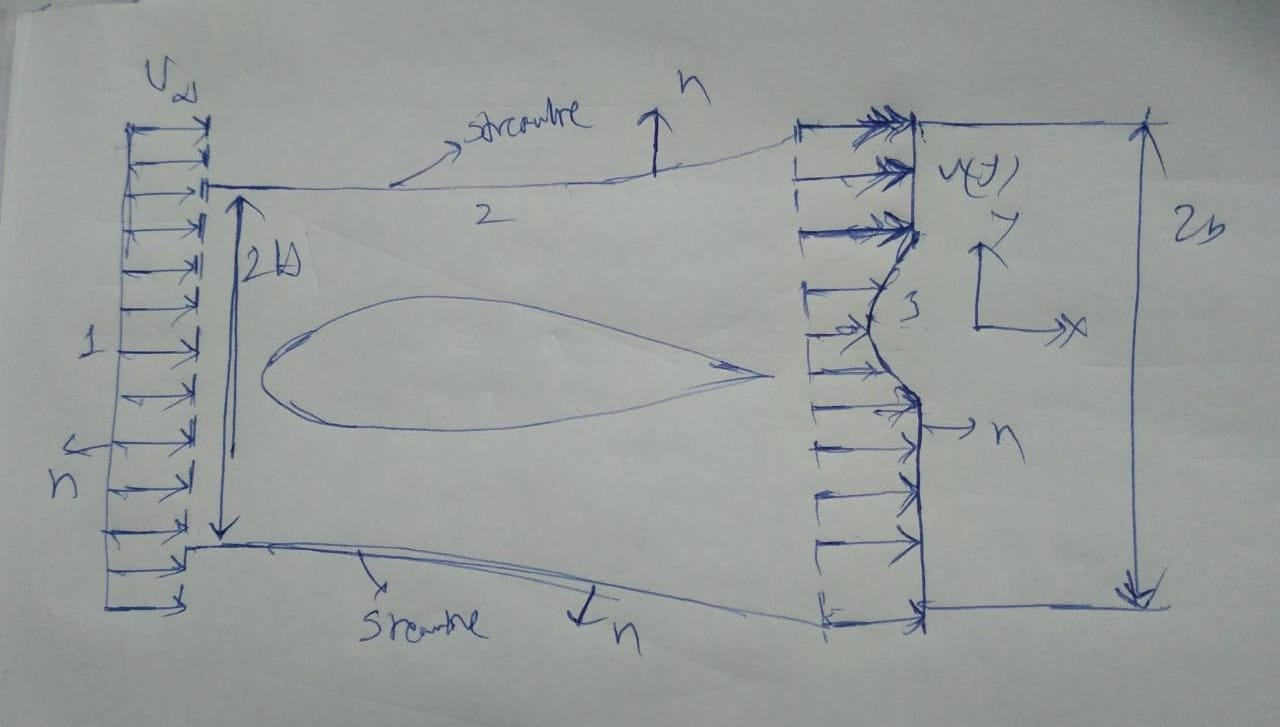
\includegraphics[scale=0.25]{8.1.jpg}
		}
	\end{center}
	\caption{Wake and Velocity profile behind a symmetric airfoil}
\end{figure}





\section{Procedure :}
\begin{enumerate}
    \item In wind tunnel test section is set.
    \item Pitot-static probe is connected to manometer.
    \item Fan speed is fixed.
    \item Required readings are taken.
\end{enumerate}






\section{Observation :}


\subsection{Wake velocity profile with distance of Pitot  probe  }
\begin{table}[ht]
\centering
\caption{\textbf{Wake profile velocity with distance of pitot probe}}
\vspace{2mm}

\begin{tabular}{|p{20mm}|p{20mm}|p{20mm}|p{25mm}|p{25mm}|} 
 \hline
Port No. & Distance from starting point(in mm) & Stagnation Pressure(in Pa) & Velocity(m/s) \\ [0.1ex] 
 \hline
$P_1$ & 0 & -3  & 14.584 \\ 
 \hline
$P_2$ & 6 & -4 & 14.528  \\
 \hline
$P_3$ & 12 & -5 & 14.472  \\
 \hline
 $P_4$ & 18 & -5 & 14.472  \\
 \hline
$P_5$ & 24 & -5 & 14.472  \\
 \hline
$P_6$ & 30 & -7 & 14.359 \\ 
 \hline
$P_7$ & 36 & -110 & 6.165 \\ 
 \hline
$P_8$ & 42 & -5 & 14.472\\
 \hline
$P_9$ & 48 & -4 & 14.528\\
 \hline
$P_{10}$ & 54 & -3 & 14.584\\ 
 \hline 
Between $P_{4}$ $\And$ $P_{5}$ & 21 & -5 & 14.472\\ 
 \hline
Between $P_{5}$ $\And$ $P_{6}$ & 27 & -5 & 14.472\\ 
 \hline
Between $P_{6}$ $\And$ $P_{7}$ & 33 & -20 & 13.600\\ 
 \hline
Between $P_{7}$ $\And$ $P_{8}$ & 39 & -22 & 13.479\\ 
 \hline
Between $P_{8}$ $\And$ $P_{9}$ & 45 & -3 & 14.584\\ 
 \hline
\end{tabular}

\end{table}

\begin{figure}[!ht]
	\begin{center}
		\framebox{
			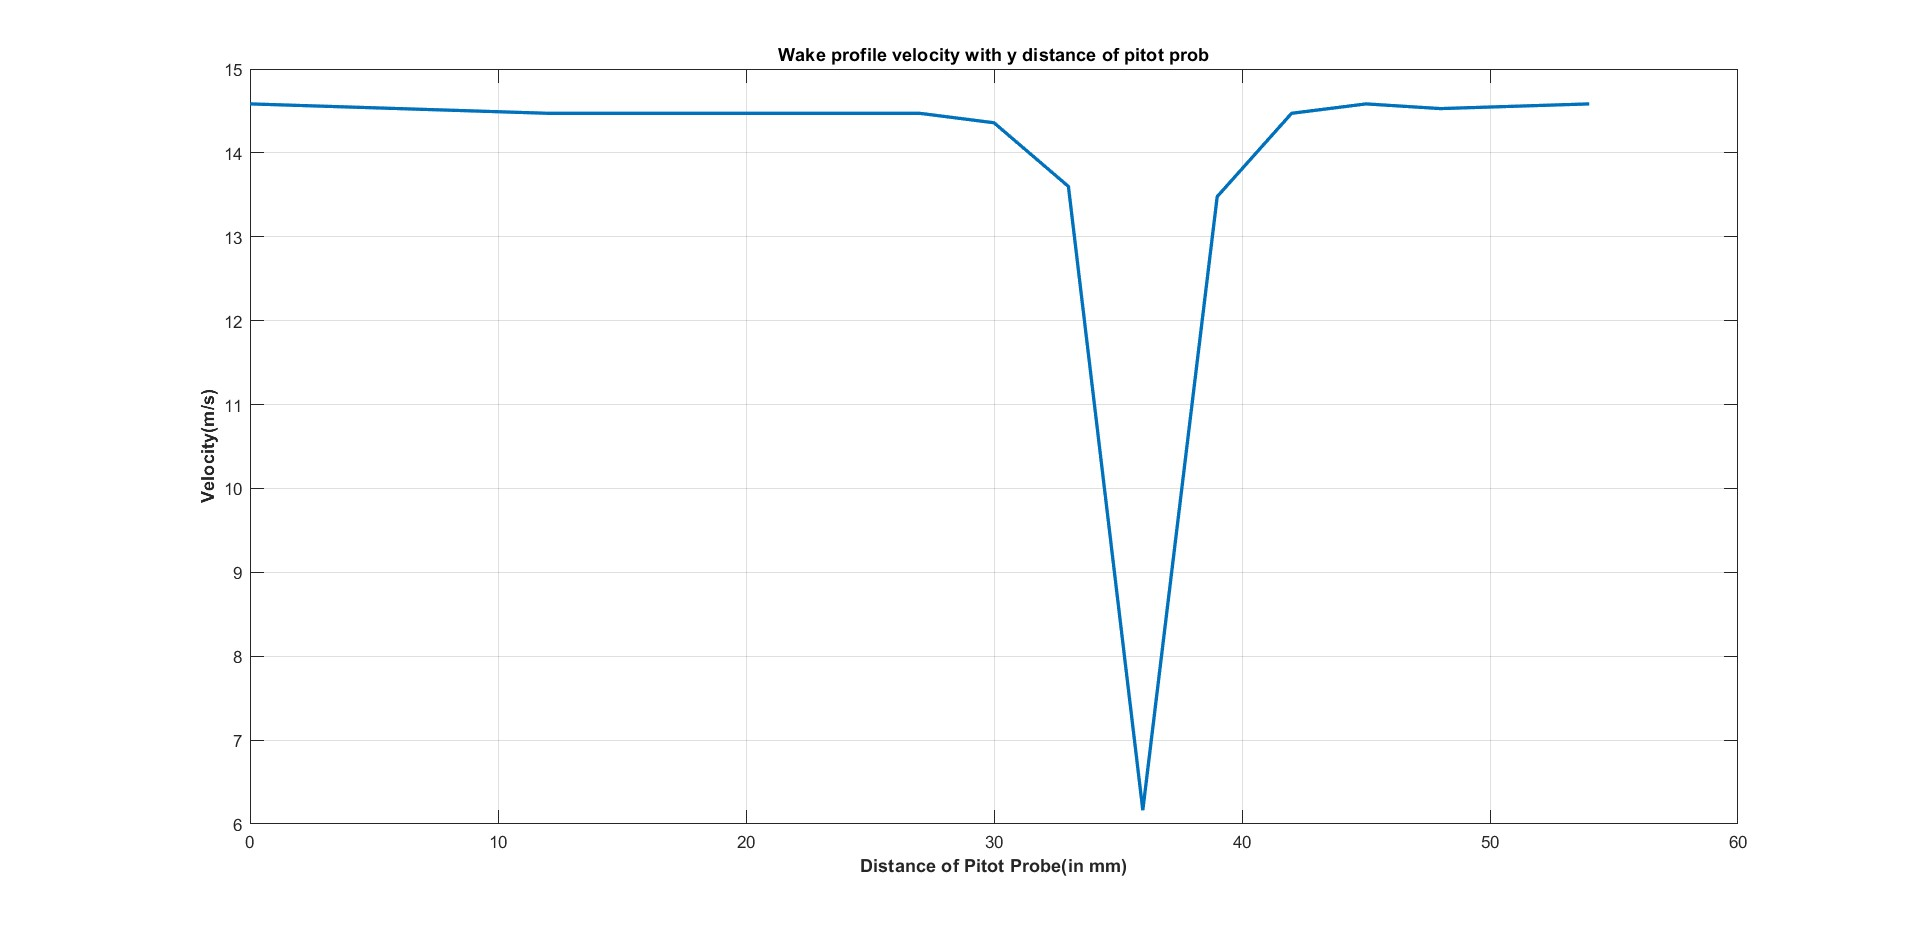
\includegraphics[scale=0.25]{vy graph.jpg}
		}
	\end{center}
	\caption{Variation of velocity with distance of pitot tube.}
\end{figure}



\newpage









\newpage

\subsection{Coefficient of Drag vs Angle of Attack : } 



\begin{table}[ht]
\centering
\caption{\textbf{Variation of Drag Coefficients with Angle of Attack}}
\vspace{2mm}

\begin{tabular}{|p{20mm}|p{20mm}|p{30mm}|p{30mm}|} 
 \hline
Sl. No. & Angle of Attack($\alpha$)  & Coeff of Drag($C_d$)(For V=15 m/s) & Coeff of Drag($C_d$)(For V=20 m/s) \\ [0.1ex] 
 \hline \hline
1 & 0 &  0.113 & 0.134 \\ 
 \hline
2 & 2 &  0.0469 & 0.027 \\
 \hline
3 & 4 &  0.0334 & 0.0602 \\
 \hline
4 & 6 &  0.0904 & 0.0652  \\
 \hline
5 & 8 &  0.0922 & 0.0762 \\
 \hline
6 & 10 &  0.1346 & 0.0538 \\ 
 \hline
7 & 12 &  0.28 & 0.0672 \\ 
 \hline


\end{tabular}
\end{table}


\begin{figure}[!ht]
	\begin{center}
		\framebox{
			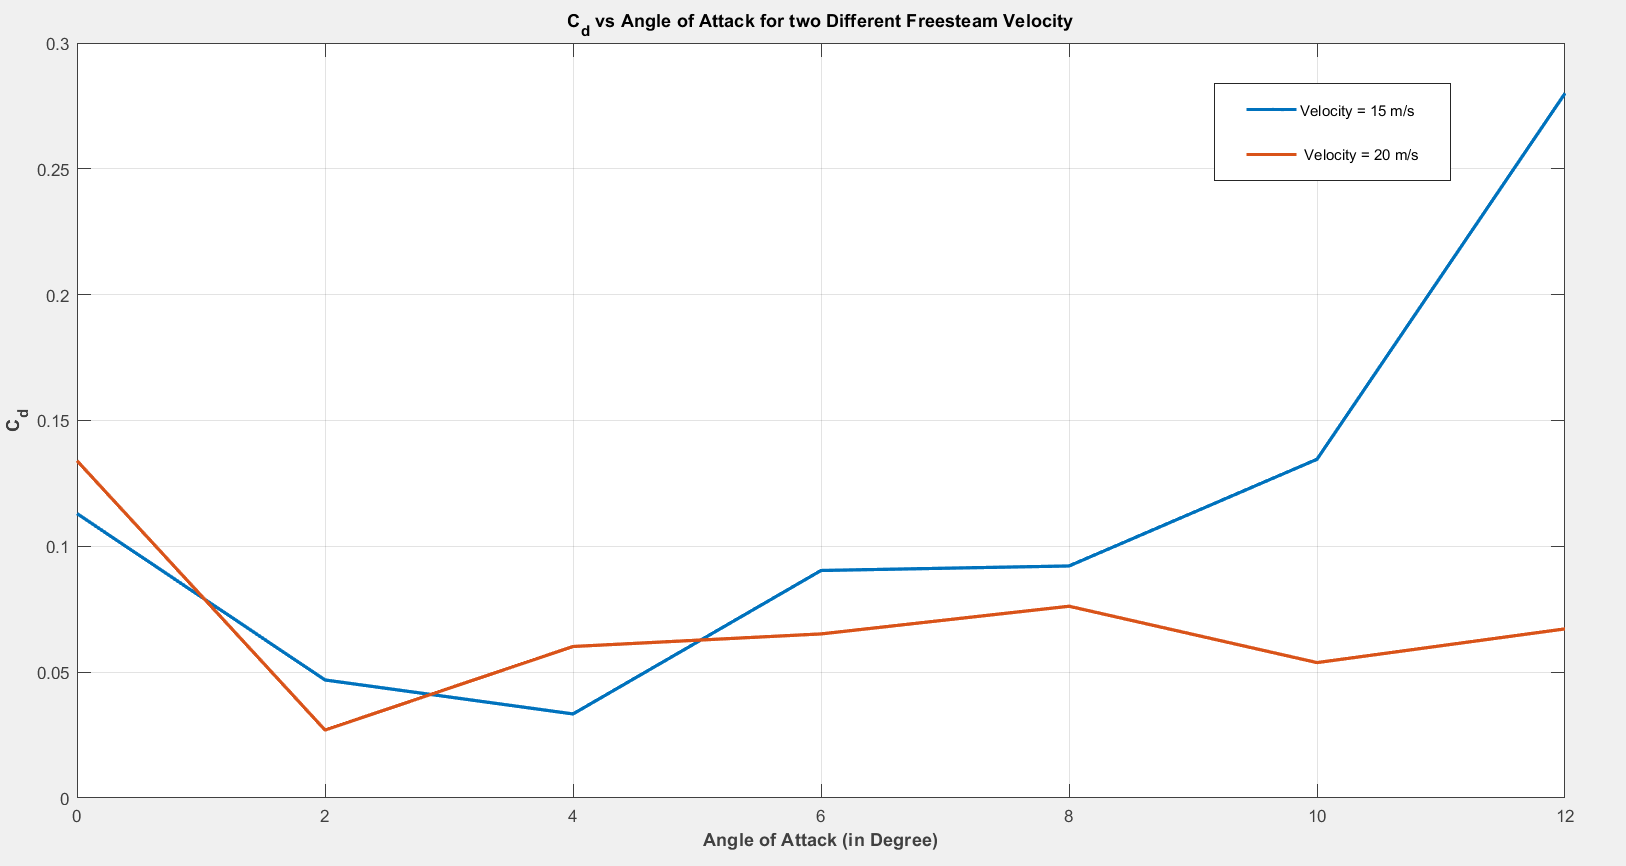
\includegraphics[scale=0.42]{cd vs aoa.png}
		}
	\end{center}
	\caption{Variation of Coefficients of Drag with Angle of Attack for Two different Velocities}
\end{figure}

\newpage














\section{Calculations :}
Density of air = 1.225 $m^3$ \\
Static Pressure($P_{\infty}$ =-13.6 mm of Water = -133.28 Pa \\
Density of Water($\rho_{w}$) = 1000 $Kg/m^3$

\subsection{Calculation of wake profile velocity :}
For port 1 : \\
Stagnation Pressure($P_{stag}$) = -3 Pa 

$$  P_{stag} = P_{\infty} + \frac{\rho v^2}{2} $$
$$\Rightarrow   P_{stag}-P_{\infty} = \frac{\rho v^2}{2}$$ 
$$\Rightarrow (133.28-3) = \frac{\rho v^2}{2} $$
$$\Rightarrow v = \sqrt{\frac{130.28\times 2}{1.225}} $$
$$\Rightarrow v = 14.584 m/s $$





\subsection{Calculation of Drag :}
Drag(D) is calculated by , \\
For 10 ports,\[ D = \int_{-\infty}^{\infty} \rho v (V_{\infty}-v)\,dy  \approx  \sum_{i=1}^{9} \rho v_{avg}(V_{\infty} - v_{avg})\Delta y \ \]
Where, $v_{avg} = \frac{v_i + v_{i+1}}{2} $ \\
$\Delta y = 6 mm = 0.006 m $ \\
$V_{\infty}$ = 15 m/s $\\


$$ D = \sum_{i=1}^{9} \rho v_{avg}(V_{\infty} - v_{avg})\Delta y $$\\
$$\Rightarrow D = 1.225 [(14.556) \times (15 - 14.556) + (14.5) \times (15 - 14.5) + (14.472) \times (15 - 14.472)  \\$$
$$ + (14.472) \times (15 - 14.472) + (14.4155) \times (15-14.4155) + (10.262) \times (15-10.262) + 
(10.3185) \times (15-10.3185) \\ $$
$$+ (14.5) \times (15-14.5) + (14.556) \times (15-14.556)] \times 0.006 \\ $$

$\therefore D = 0.150 N \\



\subsection{Calculation of Coefficients of Drag ($C_d$) and Reynolds number($R_e$):}
Chord length(c) = 65 mm\\
For velocity($V_{\infty}$) = 15 m/s, \\

$$ C_d = \frac{2D}{(\rho V_{\infty}^2 c)/2} $$


$$ \therefore C_d = 0.0334 $$



$$ R_e = \frac{\rho V_{\infty }c}{\mu} $$ \\
Where $\mu = 1.81 \times 10^{-5} $
$$ \therefore R_e = \frac{1.225\times 15 \times 0.065}{1.81\times10^{-5}} = 65987.57 $$


\section{Sources of Error:}
\begin{itemize}
    \item Error due to instrumental defect.
    \item Error may occur in taking readings before flow becomes steady.
    \item Error due to environmental effect like temperature,pressure change.
    \item Error in measurement due to presence of zero error in parameters.
    \item Dimensional error may occurs 
\end{itemize}



\section{Conclusion :}
\begin{itemize}
    \item Wake velocity profile is symmetrical.It falls suddenly at centerline then it remains almost constant as earlier.
    \item Generally Drag increases on increasing Angle of attack. 
    \item Induced Drag increases as Angle of Attack increases and it decreases when airspeed increases. But for Parasite Drag increases as airspeed increases and remains unaffected on changing Angle of Attack.
    \item Wake calculation system is a very common method for calculating Drag and Coefficient of Drag.
\end{itemize}


\end{document}